\chapter{Stability of fixed points}
Now we would like to begin to explore the behaviour of dynamical systems around fixed points. This will allow us to find out if we should expect to observe a fixed state, and to understand what happens if we perturb the system away from this fixed state.
\section{Basic definitions}
Consider
\begin{align}
	\dot{ {x}}=f( {x},t),\  {x} \in \mathbb{R}^{n},\ f\in \mathcal{C}^{1}.
\end{align}
Assume that $ {x}=0$ is a fixed point, i.e. $f({0},t) = {0}$ for all $t \in \mathbb{R}$. If the fixed point is originally at ${x}_0\neq {0}$, shift it to zero by letting $\tilde{ {x}}:= {x}- {x}_0$, therefore 
\begin{align}
	\dot{\tilde{ {x}}} = \dot{ {x}} = f( {x}_0 + \tilde{ {x}}, t) = \tilde{f}(\tilde{ {x}}, t).
\end{align}
We would like to understand how the dynamical system behaves near its equilibrium state. To this end we introduce the following definitions.
\begin{definition}[Lyapupnov Stability] \label{def:stable}
	The fixed point $ {x}={0}$ is stable if for all $t_0$, for all $\varepsilon>0$ small enough, there exists a $\delta=\delta(t_0, \varepsilon)$, such that for all $ {x}_0 \in \mathbb{R}^{n}$ with $\| {x}_0\| \leq \delta$, we have 
	\begin{align}
		\boxed{
			\left \|  {x}(t;t_0,  {x}_0) \right\| \leq \varepsilon \quad \forall t \geq t_0.
		}
	\end{align}
\begin{figure}[h!]
	\centering
	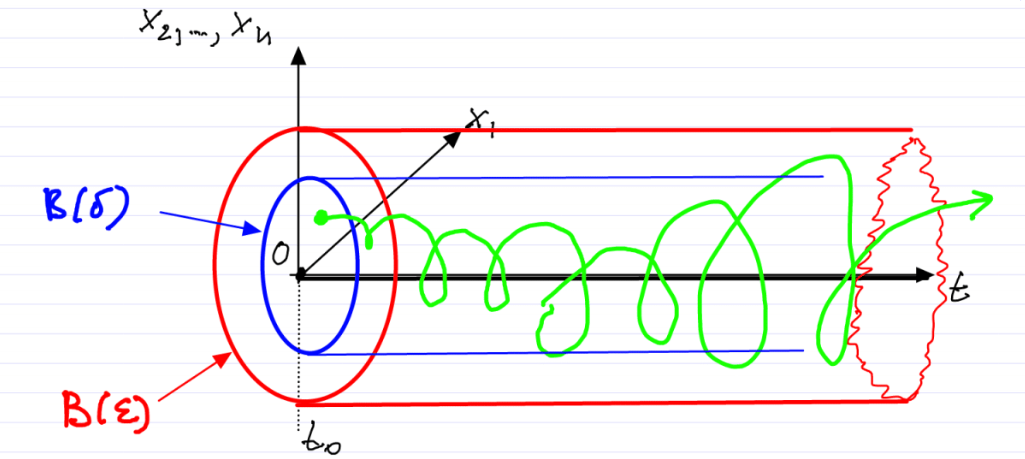
\includegraphics[width=0.7\textwidth]{figures/ch2/1lyapunov_stability.png}
	\caption{An example such a $\delta$ for a given Lyapunov stable fixed point.}
	\label{fig:lyapunov_stability_def}
\end{figure}
\end{definition}
\begin{remark}[N-dimensional ball]
	When writing $\mathcal{B}(r)$ we refer to the ball of radius $r$ in $\mathbb{R}^{n}$, i.e. the set $\{x:\ \|x\| < r\}$.
\end{remark}

\begin{ex}[Stability of the lower equilibrium of the pendulum]
	Recall the equation of motion of the pendulum $\ddot{\varphi} + \sin(\varphi) = 0$, that we transform into a first order ODE by setting $x_1 = \varphi$ and $x_2 = \dot{\varphi}$ to obtain
	\begin{align}
		\begin{dcases}
		\dot{x}_1 = x_2 \\
	\dot{x}_2 = -\sin(x_1).
		\end{dcases}
	\end{align}
	For small $\varepsilon>0$, this geometric procedure gives a $\delta(\varepsilon)>0$ such that the definition of stability is satisfied for $ {x}=0$. We can see in Fig. \ref{fig:pend_lower_stability} that for any initial point chosen within the blue circle, it's trajectory remains within the red circle for all time (cf. Fig. \ref{fig:lyapunov_stability_def}). Therefore $ {x}=0$ is (Lyapunov) stable.
	\begin{figure}[h!]
		\centering
		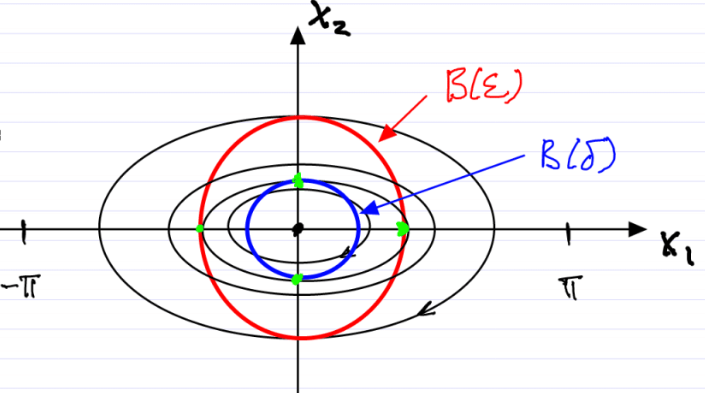
\includegraphics[width=0.5\textwidth]{figures/ch2/2pendulum_stability.png}
		\caption{Stability of lower equilibrium for the pendulum, here $0<\varepsilon<\pi $.}
	\label{fig:pend_lower_stability}
	\end{figure}
\end{ex}

\begin{definition}[Asymptotic stability]
	The fixed point $ {x}=0$ is \emph{asymptotically stable} if
\begin{enumerate}
	\item it is stable,
	\item for all $t_0$, there exists $\delta_0(t_0, \varepsilon)$ such that for every $ {x}_0$ with $\|  {x}_0 \| \leq \delta_0$ we have
		\begin{align}
			\boxed{\lim_{t\to \infty }  {x}(t; t_0,  {x}_0) = 0.}
		\end{align}
\end{enumerate}
\begin{figure}[h!]
	\centering
	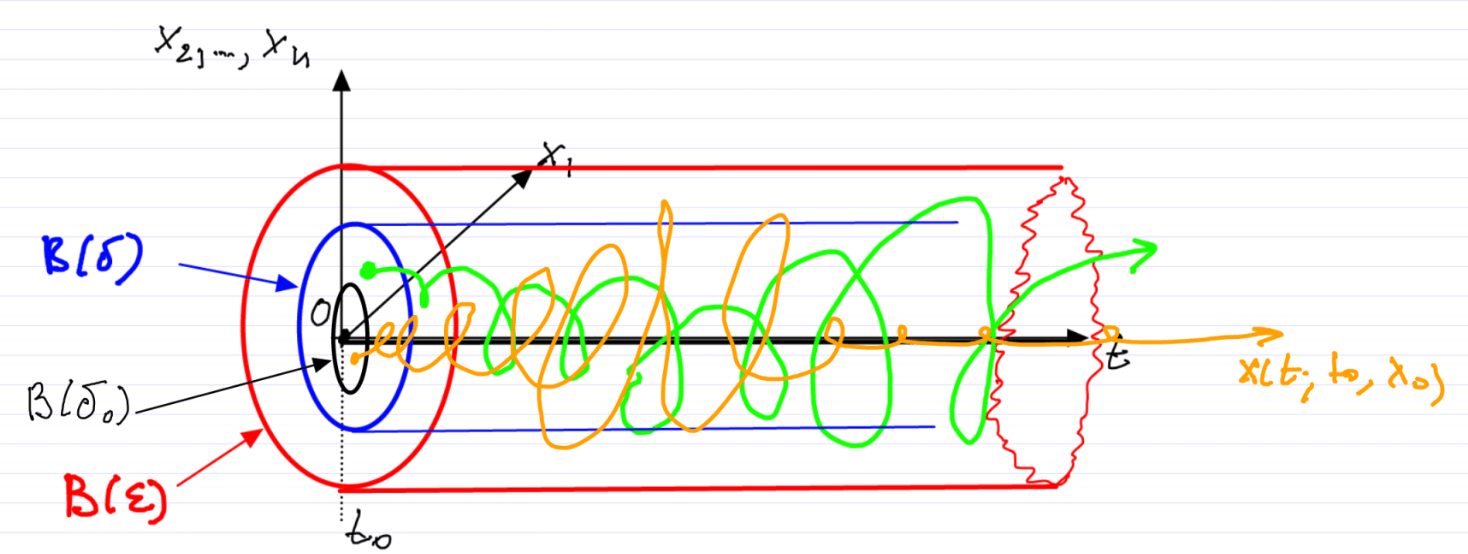
\includegraphics[width=0.7\textwidth]{figures/ch2/3asymp_stability.png}
	\caption{An example for an asymptotically stable fixed point (black trajectory).}
\end{figure}
\end{definition}

\begin{definition}[Domain of attraction] 
	The \emph{domain of attraction} of the fixed point $x=0$ is the set of all $ {x}_0$'s for which
	\begin{align}
		\boxed{\lim_{t\to \infty } {x}(t;t_0,  {x}_0)=0. }	
	\end{align}
	
\end{definition}

\begin{ex}[Damped pendulum]
	We have the equation of motion with the linear damping coefficient $c$
	\begin{align}
		\ddot{\varphi} + c \dot{\varphi} + \sin(\varphi) = 0,\quad c>0.
	\end{align}
	Transforming into a first-order ODE with $x_1 = \varphi$ and $x_2 = \dot{\varphi}$ gives
	 \begin{align}
		\begin{dcases}
		\dot{x}_1 = x_2\\ \dot{x}_2 = -cx_2 - \sin(x_1).
		\end{dcases}
	\end{align}
The total energy is given by
\begin{align}
	E = \frac{1}{2}x_2^2 + \left( 1 - \cos(x_1) \right). 
\end{align}
Further we have the rate of energy change
\begin{align}
\frac{d}{dt} E(x_1(t), x_2(t)) = x_2 \left(\dot{x}_2 + \sin(x_1) \right) = -c x_2^{2}.
\end{align}
\begin{figure}[h!]
	\centering
	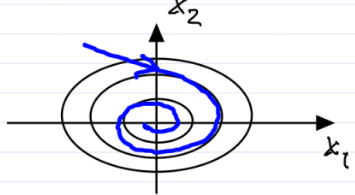
\includegraphics[width=0.35\textwidth]{figures/ch2/4damped_pendulum.png}
	\caption{An example of a trajectory which loses energy, in this case due to damping.}
	\label{fig:losing_energy_pend}
\end{figure}

Therefore, along trajectories energy decreases monotonically as shown in Fig \ref{fig:losing_energy_pend}. By the $\mathcal{C}^0$ dependence of the trajectory on initial conditions, the trajectories remain close to the undamped oscillations for small $c>0$. We conclude that trajectories are inward spirals for a small dissapation $c>0$. The fixed point $ {x}=0$ is still Lyapunov stable, but asymptotic stability does not yet follow (is the limit of $ {x}(t)$ equal to 0?).
\begin{remark}[LaSalle's invariance principle]
	This conclusion follows rigorously from LaSalle's invariance principle, namely if we assume that $\dot{ {x}}=f( {x})$, $f \in \mathcal{C}^1$, and that there exists a $V\in \mathcal{C}^1$ with 
	\begin{align}
		\dot{V} = \frac{dV( {x}(t))}{dt} \leq 0.	
	\end{align}
	Then the set of accumulation points for any trajectory is contained in the set of trajectories that stay within the set $I=\{ {x} \in \mathbb{R}^{n}:\ \dot{V}( {x}) = 0\}$.
\end{remark}
\end{ex}

\begin{ex}[]
	Consider the following dynamical system in polar coordinates, i.e. $r\cos(\theta) = x$ and $r \sin(\theta) = y$,
	\begin{align}
		\begin{dcases}
			\dot{r} = r(1-r) \\ \dot{\theta} = \sin^2\left( \frac{\theta}{2} \right).
		\end{dcases}
	\end{align}
	Note that $r=0$ is a fixed point, the set $r=1$ is an invariant circle, and the set $\theta=0$ is an invariant set. An invariant set is a set such that if the dynamical system is started on the set, it remains in the set for all time. Examining the radial evolution reveals that the equation of motion decouples. We see that $\dot{\theta}\geq 0$, so rotation is either positive or null.
	\begin{figure}[h!]
		\centering
		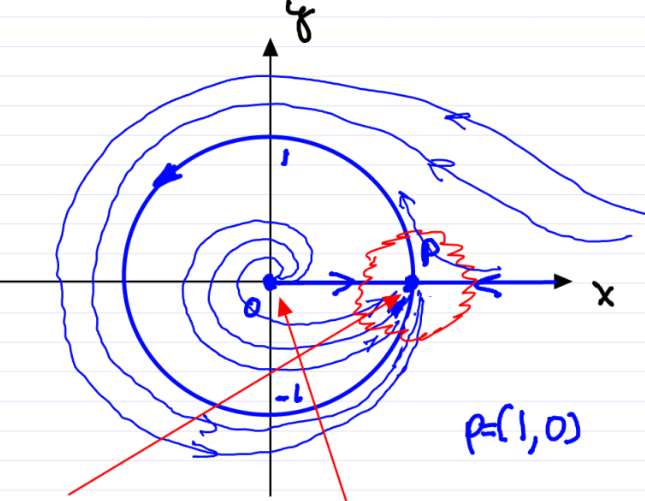
\includegraphics[width=0.5\textwidth]{figures/ch2/5polar_cds.png}
		\caption{Phase portrait of the dynamical system in cartesian coordinates, with the red arrows pointing to the two unstable equilibria.}
		\label{fig:polar_attractor}
	\end{figure}

	 From Fig. \ref{fig:polar_attractor} we can see that both of the fixed points, $(0,0)$ and $(1,0)$, are not stable. However, inspecting Fig. \ref{fig:polar_attractor} we see that that $p=(1,0)$ is an example of an attractor: a set with an open neighborhood of points that all approach the set as $t\to \infty $.
\end{ex}

\begin{definition}[Invariant set]
	The set $S \subset P$ is an \emph{invariant set} for the flow map $F^{t}:P \to P$ if $F^{t}(S) =S$ for all $t \in \mathbb{R}$.
\end{definition}

\begin{definition}[Unstable point]
	A fixed point $ {x}=0$ is unstable if it is not stable.
\end{definition}

\begin{remark}[]
	We can negate a mathematical statement by using the reverse relational operators outside the statements involving these operators i.e. $ \exists \to \forall $ and $\forall \to \exists $. For example we have for continuity $\forall \varepsilon\ \exists \delta:\  \|f( {x}) - f( {y}) \| < \varepsilon$ if $ \| {x}- {y} \|<\delta$, meanwhile for discontinuity we have  $\exists \varepsilon:\ \forall \delta:\  \|f( {x}) - f( {y}) \| \geq  \varepsilon$ for $ \| {x}- {y} \|< \delta$.

	In our case for stability we have
	\begin{align}
		\forall \varepsilon,t_0: \quad \exists \delta>0: \quad \forall  {x}_0  \textrm{ with }  \| {x}_0 \| < \delta: \quad  \| {x}(t) \|\leq \varepsilon \quad \forall t\geq t_0.
	\end{align}
Meanwhile for instability 
\begin{align}
	\exists \varepsilon,t_0:\quad \underbrace{\forall \delta>0}_{ \textrm{``for arbitrarily small"} }:\quad \exists  {x}_0  \textrm{ with }  \| {x}_0 \|<\delta: \quad  \| {x}(t) \|>\varepsilon \quad \underbrace{\exists t\geq t_0}_{ \textrm{``for some"} }.
\end{align}
This negation is demonstration in Fig. \ref{fig:instable_def}.
\begin{figure}[h!]
	\centering
	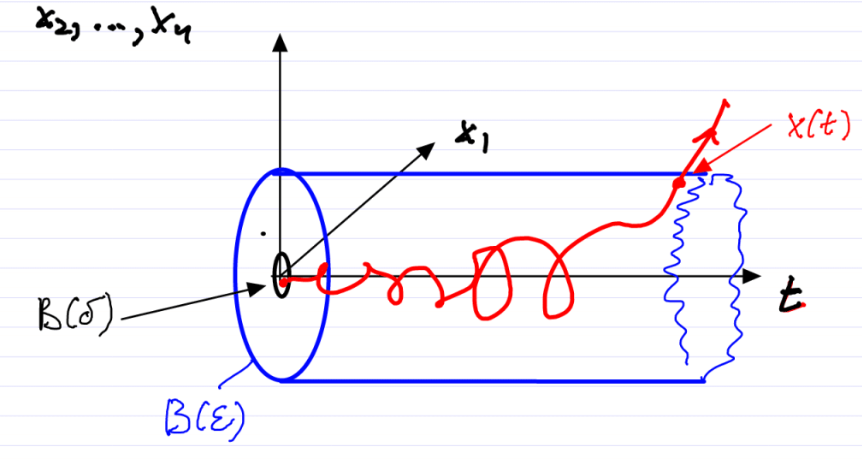
\includegraphics[width=0.5\textwidth]{figures/ch2/6unstable_def.png}
	\caption{Example of an unstable fixed point, with the red trajectory representing a trajectory starting arbitraritly close to the fixed point, leaving a given $\varepsilon$-ball.}
	\label{fig:instable_def}
\end{figure}
\end{remark}

\begin{remark}[]
	By $\mathcal{C}^0$ dependence of trajectories on initial conditions, if $ {x}(t;t_0, {x}_0)$ leaves $\mathcal{B}(\varepsilon)$, then for $\tilde{ {x}}_0$ close enough to $ {x}_0$, $ {x}(t;t_0,\tilde{ {x}}_0)$ also leaves $\mathcal{B}(\varepsilon)$. Since this is true on an open set around ${x}_0$, the measure of such trajectories in nonzero, the instability is observable!
\end{remark}

\begin{ex}[Unstable fixed point of pendulum]
	In contrast, we can have that infinitely many trajectories converge to the fixed point, yet it is still unstable, as illustrated in Fig. \ref{fig:convergent_unstable}. In fact, the converging trajectories form a measure-zero set, thus the stability near the unstable equilibrium is unobservable.
	\begin{figure}[h!]
		\centering
		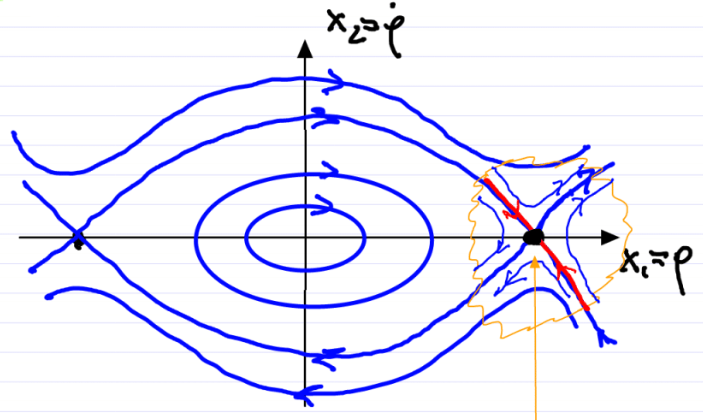
\includegraphics[width=0.6\textwidth]{figures/ch2/7unstable_pendulum.png}
		\caption{The phase portrait around the unstable fixed point of the pendulum, with the stable trajectories (red).}
		\label{fig:convergent_unstable}
	\end{figure}
	
\end{ex}
\newpage
\section{Stability based on linearization}
We would like to derive a more general method to analyze the stability of fixed points, thus we try to simplify our system around the fixed point and discover what this can tell us about the full (unsimplified) system. In the following section we shall always assume that our system is autonomous. We will have the following setup
\begin{align*}
	\dot{ {x}}=f( {x}),\quad f\in \mathcal{C}^1,\quad  {x}=
	\begin{pmatrix}
		x_1\\ \vdots \\ x_n
	\end{pmatrix}\in \mathbb{R}^{n}, \quad 
	{p} = 
\begin{pmatrix}
	p_1 \\ \vdots \\ p_n 
\end{pmatrix}
\in \mathbb{R}^{n}. \numberthis \label{eq:star}
\end{align*}

If $f({p} )={0} $, then ${p} $ is a fixed point. By transforming using ${y} = {x} - {p} $, we have that in the transformed system ${y} = {0} $ is a fixed point. Furthermore, we have that around ${y} = {0} $ the ODE is 
\begin{align}
	\dot{{y} } = f({p} + {y} ) = \underbrace{f({p} )}_{=0} + Df({p} ){y} + o(\| {y} \|) = Df({p} ){y} + o(\| {y} \|).
\end{align}
\begin{remark}[]
	Since we only assumed one continuous derivative for the function $f$ the remainder term in the Taylor approximation is $o(\|y\|)$. The little o notation means that 
	\begin{align}
		\lim_{\|y\| \to 0} \frac{o(\|y\|)}{\|y\|}=0.
	\end{align}
	
\end{remark}

\begin{definition}[Linearized ODE]
	We define the \emph{linearization} of \eqref{eq:star} at the fixed point ${p} $ as 
	\begin{align*}
		\boxed{
		\dot{{y} } = {A} {y}; \quad {y} \in \mathbb{R}^{n},\quad {A} := Df({p} ) \in \mathbb{R}_{n \times n};\quad  Df(p) = 
	\left. \begin{pmatrix}
		\frac{\partial f_1}{\partial x_1} & \ldots & \frac{\partial f_1}{\partial x_n} \\
		\vdots & & \vdots \\
		\frac{\partial f_n}{\partial x_1} & \ldots & \frac{\partial f_n}{\partial x_n}
\end{pmatrix}\right|_{{x} = {p} }.} \numberthis \label{eq:sstar}
	\end{align*}
\end{definition}
Now we would like to study the stability of the fixed point ${y} =0$ in \eqref{eq:sstar}. From this analysis, we want to know the relevance of our results for the full nonlinear system \eqref{eq:star}.

\section{Review of linear dynamical systems}
Recall the setup
\begin{align}
	\dot{{y} } = {A} (t){y}, \quad {y} \in \mathbb{R}^{n}, \quad {A} \in \mathbb{R}^{n \times n}, \quad {A} \in \mathcal{C}^{0}_{t}.
\end{align}
The following facts have already been established
\begin{itemize}
	\item We know that the global existence and uniqueness of solutions is guaranteed. 
	\item The superposition principle holds; namely the linear combination of solutions is also a solution.
	\item There exists a set of $n$ linearly independent solutions: $\varphi_1(t), \ldots, \varphi_n(t) \in \mathbb{R}_{n}$.
	\item The general solution is
		\begin{align}
			y(t) = \sum_{i=1}^{n} c_i \varphi_i(t) =
			\underbrace{\begin{bmatrix}
				\varphi_1(t) & \ldots & \varphi_n(t)
		\end{bmatrix}}_{\Psi(t):  \textrm{ fundamental matrix solution} }
		\underbrace{\begin{bmatrix}
			c_1 \\ \vdots \\ c_n
	\end{bmatrix}}_{c}
	= \Psi(t) {c}; \quad \dot{\Psi} = A(t) \Psi.			
		\end{align}
	\item We have the initial value problem ${y} (t_0) = {y} _0$ which implies
		\begin{align}
			\Psi(t_0) {c} = {y} _0 \implies {y} (t) = \underbrace{\Psi(t) \left[\Psi(t_0)\right]^{-1}}_{\phi(t):= F_{t_0}^{t}}{y} _0 
		\end{align}
		Where we used that the $\varphi_i(t)$ are linearly independent in the last equality. And we have the \emph{normalized fundamental matrix} $\phi(t)$ equal to the flow map, with $\phi(t_0)={I} $.
	\item In the autonomous case $\dot{{x} }= {A} {x} $ solutions can be practically constructed.
	\begin{enumerate} 
		\item \textbf{Explicit Solution} 
		\begin{align}
			\phi(t) = e^{{A} t} := \sum_{j=0}^{\infty } \frac{1}{j!} ({A} t)^{j}
		\end{align}
	With $0! =1$ and ${0} ^{0}= {I} $. We can verify that this is indeed a solution
	\begin{align}
		\dot{\phi}(t) = \sum_{j=1}^{\infty } \frac{1}{(j-1)!} ({A} t)^{j-1}{A} = {A} \sum_{j=0}^{\infty } \frac{1}{j!} ({A} t)^{j} = {A}  e^{{A} t} = {A} \phi(t).
	\end{align}
	Where we used that ${A} $ commutes with its powers in the second equality. We now have that each column of $\phi(t)$ satisfies $\dot{{y} } = {A} {y} $.	
	\begin{remark}[]
		For a scalar ODE $\dot{y}= a(t)y$ for $y \in \mathbb{R}$, the solution is known $y(t) = e^{\int_{t_0}^{t} a(s)ds}y_0$. However, this does not extend to the higher dimensional $\dot{{y} }= {A} (t){y} $. In fact, in general, $\phi(t) = e^{\int_{t_0}^{t} {A} (s)ds}$ is \underline{not} a solution. We can check this
	\begin{align}
		\dot{\phi} = \sum_{j=0}^{\infty } \frac{1}{j!} \frac{d}{dt} \left( \int_{t_0}^{t} {A} (s) ds \right)^{j} = \sum_{j=1}^{\infty } \frac{1}{(j-1)!} \left( \int_{t_0}^{t} {A} (s)ds \right)^{j-1} {A} (t) \neq {A} (t) \phi(t).
	\end{align}
	The nonequality holds as ${A} (t)$ does not generally commute with $\int_{}^{} {A} (s)ds$.
	\end{remark}

\item \textbf{Solution from eigenfunctions} If we have an autonomous system, we can solve the ODE without an infinite series. We have 
	\begin{align*}
		\dot{{y} } = {A} {y} ,\quad {y} \in \mathbb{R}^{n}, \quad {y} (0) = {y}_0. \numberthis \label{eq:onestar}
	\end{align*}
	Substituting $\varphi(t)=e^{\lambda t}{s} $ for $\lambda\in \mathbb{C}$ and ${s} \in \mathbb{C}^{n}$ into \eqref{eq:onestar} yields
\begin{align*}
	\lambda {s} = {A} {s} \implies ( {A} - \lambda {I} ) {s} = 0 \iff \det( {A} - \lambda {I} ) = 0 \numberthis \label{eq:twostar}.
\end{align*}
Therefore $\lambda$ must be an eigenvalue of ${A}$ and ${s} $ must be the corresponding eigenvector. We call $\det({A} - \lambda {I} )$ the \emph{characteristic equation} of ${A} $. Let $\lambda_1, \ldots , \lambda_n$ be the eigenvalues and ${s} _1, \ldots, {s} _n$ be the corresponding eigenvectors. In the case that some eigenvalues are repeated, some of the ${s} _i$ may be generalized eigenvectors. We then have two cases.
\begin{enumerate}
	\item ${A} $ is semisimple, i.e. the eigenvectors are linearly independent (which is always the case if the $\lambda_i$ all have algebraic multiplicity of one). Then we have the solution
		\begin{align}
			{y} (t) = \sum_{i=1}^{n} c_i e^{\lambda_i t}{s} _i = \sum_{j=1}^{n} c_j e^{ (\textrm{Re} \lambda_j) t} e^{i( \textrm{Im} \lambda_j)t} {s} _j.
		\end{align}
	Where we used $\lambda_j =  \textrm{Re} \lambda_j + i  \textrm{Im} \lambda_j$.	
\item ${A} $ is \underline{not} semisimple, i.e. has repeated eigenvalues (but not enough linearly independent eigenvectors). Then we assume that $\lambda_k$ has algebraic multiplicity $a_k > g_k$, where $a_k$ measures the multiplicity of $\lambda_k$ as a root of $\det({A} - \lambda {I} )=0$, and $g_k$ is the number of linearly independent eigenvectors for $\lambda_k$, also called the \emph{geometric muliplicity} of $\lambda_k$. Even in this case, $\lambda _k$ gives rise to $a_k$ linearly independent solutions of the form
	\begin{align}
		\underbrace{{P} _0}_{={s_k} } e^{\lambda _k t},\ {P} _1(t) e^{\lambda _k t}, \ {P}_2(t)e^{\lambda _k t}, \ldots, {P} _{a_{k-1}}(t)e^{\lambda _k t}
	\end{align}
	where ${P} _{j}(t)$ is a vector polynomial of $t$ of order $j$ or less.	
\end{enumerate}

	\end{enumerate}
\end{itemize}

\section{Stability of fixed points in autonomous linear systems}
First we note that we can bound our solution
\begin{align*}
	\| {y} (t) \| = \| \phi(t) {y} _0 \| \leq \underbrace{\| \phi(t) \|}_{ \textrm{Operator norm} } \| {y}_0 \| \leq C e^{\mu t} \| {y} _0 \|. \numberthis \label{eq:1star}
\end{align*}
Where $\mu = \max_j ( \textrm{Re} \lambda_j) + \nu $, with $\nu >0$, as small as needed, provided we increase $C$ appropriately. If ${A} $ is semisimple, then $\nu =0$ can be selected.
\begin{theorem}[Stability of fixed points in linear systems] \label{thm:lin_stab_eigv}
	Given ${y} =0$ a fixed point of the linear system $\dot{{y} } = {A} {y} $ with ${A} \in \mathbb{R}^{n \times n}$ the following statements hold:
	\begin{enumerate}
		\item Assume that $ \textrm{Re} \lambda _j < 0$ for all $j$. Then ${y} =0$ is asymptotically stable.
		\item Assume that $ \textrm{Re} \lambda _j \leq 0$ for all $j$, and for all $\lambda_k$ with $ \textrm{Re} \lambda_k = 0$ we have $a_k = g_k$. Then ${y} =0$ is stable.
		\item Assume there exists a $k$ such that $ \textrm{Re} \lambda _k >0$. Then ${y} =0$ is unstable.
	\end{enumerate}
	These scenarios are illustrated in Fig. \ref{fig:eigv_setup}.
\end{theorem}
\begin{proof}
	\begin{enumerate}
		\item Pick $\varepsilon > 0$, and select $\nu > 0$ small, such that $\mu <0$. Then pick $C> 0$ such that \eqref{eq:1star} holds, and let $\delta = \frac{\varepsilon}{C}$. This implies (since $\| {y} _0\| \leq \delta $) that
			\begin{align}
				\| {y} (t) \| \leq \varepsilon e^{\mu t} \leq \varepsilon,
			\end{align}
		and
		\begin{align}
			\| {y} (t) \| \leq \varepsilon e^{\mu t} \xrightarrow{t \to \infty } 0. 
		\end{align}
	Where the limit holds as $\mu < 0$.	
\item Again choose $\delta = \frac{\varepsilon}{C}$ and note that $\mu  = \max_{j} ( \textrm{Re} \lambda _j) + \nu = 0 + \nu =0$ ($\nu =0$ as $a_k = g_k$). Then stability follows by \eqref{eq:1star}. However, asymptotic stability does not hold, as $\varphi(t) = C e^{i ( \textrm{Im} \lambda _j)t} $ solutions exist.

\item There exists a solution of the form
	\begin{align}
		{	\varphi}(t) = C_k e^{\lambda _k t} {s} _k = C_k e^{( \textrm{Re}  \lambda _k)t} e ^{i ( \textrm{Im} \lambda _k)t}{s} _k.
	\end{align}
In turn this implies
\begin{align}
	\| {\varphi}(t) \| = C_k e^{( \textrm{Re} \lambda_k) t} \| {s} _k \| \xrightarrow{t \to \infty} \infty .
\end{align}

	\end{enumerate}
\end{proof}
\begin{figure}[h!]
	\centering
	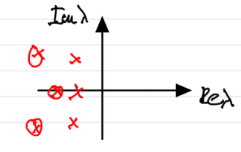
\includegraphics[width=0.3\textwidth]{figures/ch2/8eigv_setup1.png}
	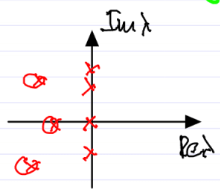
\includegraphics[width=0.3\textwidth]{figures/ch2/9eigv_setup2.png}
	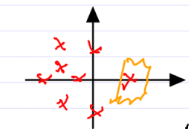
\includegraphics[width=0.3\textwidth]{figures/ch2/10eigv_setup3.png}
	\caption{Eigenvalue arrangements for scenarios (i), (ii), and (iii) (from left to right) in Theorem \ref{thm:lin_stab_eigv}}
	\label{fig:eigv_setup}
\end{figure}

\begin{ex}[Stability analysis of 2 degrees of freedom coupled oscillators]
	Given a rectangular mass $m$ with a spring of stiffness coefficient $k$ attached to each side extending to fixed walls in each cardinal direction. We want to know the stability of the equilibrium where all of the springs are equally extended. This dynamical system is depicted in Fig. \ref{fig:quad_spring}.
\begin{figure}[h!]
	\centering
	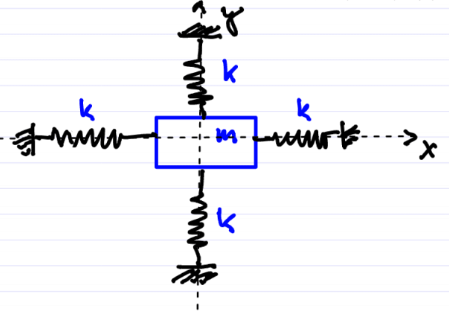
\includegraphics[width= 0.3\textwidth]{figures/ch2/11quad_spring.png}
\caption{Arrangement of coupled oscillators with rectangular mass in the middle.} \label{fig:quad_spring}
\end{figure}
First, note that this is a conservative system, i.e. $E=$ const. Next we transform the coordinates so that the equations of motion can be brought into the form of an ODE for this dynamical system
\begin{align}
	{x} = 
	\begin{pmatrix}
		x \\ \dot{x} \\ y  \\ \dot{y}
	\end{pmatrix}.
\end{align}
Thus we have a 4-dimensional, nonlinear, system of ODEs. We now linearize this at the fixed point $(x,y)= (0,0)$, i.e. $\dot{{x}} = {A} {x} $ with ${x} \in \mathbb{R}^{n}$.

The system exhibits full spatial symmetry in $x$ and $y$, hence the eigenmodes will be the same in the $x$ and $y$ directions. This means we have repeated pairs of purely imaginary eigenvalues for ${A} $:  $\lambda_{1,2}=\lambda_{3,4}= \pm i \omega $. It is clear that scenarios (i) and (iii) of Theorem \ref{thm:lin_stab_eigv} do not apply to the linearized ODE. So we need to check if (ii) applies.

We have that $ \textrm{Re} \lambda _{k}=0$ for $k=1,2,3,4$. Also $a_k=2$ for $k=1,2,3,4$. Now assume $g_k < 2$. Then there would exists solutions of the form $te^{\pm i \omega t}{s}_k$, but this would contradict the conservation of energy, as either the (nonnegative) kinetic energy and/or the (nonnegative) potential energy would grow unbounded. Hence, the total energy could not be conserved. Therefore we know that $g_k = a_k$ and we can apply (ii) to find $x=y=0$ is Lyapunov stable for the linearized system. What does this imply for the nonlinear system?
\end{ex}

\section{Stability of fixed points in nonlinear systems}
Following the previous example, we would like to know what information about the stability of fixed points of nonlinear systems we can derive from the linearized system. The full nonlinear system is
\begin{align*}
	\dot{{x} } = f(x),\quad f({x} _{0}) = {0}, \quad {x} \in \mathbb{R}^{n}, \quad f \in \mathcal{C}^{1}. \numberthis \label{eq:unostar}
\end{align*}
And its linearization at the fixed point ${x} _0$ 
\begin{align*}
	\dot{{y} } = Df({x} _0){y}, \quad y\in \mathbb{R}^{n},\quad Df({x} _0) \in \mathbb{R}^{n\times n}
	\numberthis \label{eq:dosstar}.
\end{align*}
We would like to conclude that the linearized dynamics are qualitatively similar to the nonlinear dynamics. In order to study if this is the case, we have to formalize \emph{similar} mathematically.

\begin{definition}[$\mathcal{C}^k$ equivalence of dynamical systems]
Consider two autonomous dynamical systems:
\begin{enumerate}
	\item
		\begin{align*}
			\dot{{x} }=f({x}),\quad {x} \in \mathbb{R}^{n}, \quad f \in \mathcal{C}^{1};\quad F^{t}: {x_0} \mapsto {x} (t;{x} _0). \numberthis \label{eq:uno}
		\end{align*} 
	\item	
		\begin{align}
			\dot{{x} }=g({x}),\quad {x} \in \mathbb{R}^{n}, \quad g \in \mathcal{C}^{1};\quad G^{t}: {x_0} \mapsto {x} (t;{x} _0).
		\end{align}
\end{enumerate}
The two dynamical systems are \emph{$\mathcal{C}^k$ equivalent}, for $k \in \mathbb{N}$, on an open set $U \subset \mathbb{R}^{n}$, if there exists a $\mathcal{C}^k$ diffeomorphism $h: U \to U$ that maps orbits of (i) into orbits of (ii), while preserving the orientation but not necessarily the exact parameterization of the orbit by time. Specifically for all $x\in U$, any $t _1 \in \mathbb{R}$  there exists a $t_2 \in \mathbb{R}$ such that
\begin{align}
	\boxed{
		h(F^{t_1}({x})) = G^{t_2}(h(x)).
	}
\end{align}
$h:U\to U$ does this for all $x\in U$ in a $\mathcal{C}^{k}$ fashion. This equivalence through a function $h$ is demonstrated in Fig \ref{fig:ck_equiv}.
\begin{figure}[h!]
	\centering
	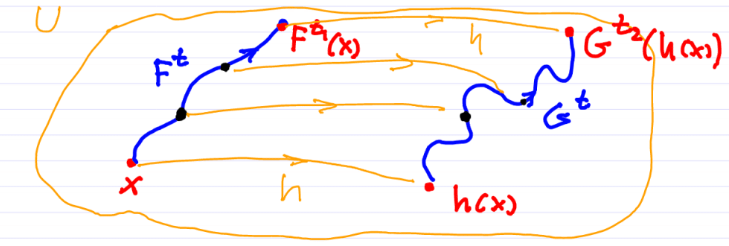
\includegraphics[width=0.7\textwidth]{figures/ch2/12ck_equiv.png}
	\caption{The function $h$ mapping the orbits of the dynamical system describing $F$ into the system describing $G$.}
	\label{fig:ck_equiv}
\end{figure}
\end{definition}
\begin{proposition}[Restrictiveness of smooth equivalence]
	Consider two $\mathcal{C}^{k}$-equivalent dynamical systems for $k>0$ with the right hand sides $f$ and $g$, as in the definitions above. Let $x_0$ be a fixed point of $F$ and $y_0$ a fixed point of $G$ such that these correspond to each other under the $\mathcal{C}^k$ equivalence, i.e. $y_0 = h(x_0)$. The eigenvalues of $Df(x_0)$ must be constant, positive multiples of the eigenvalues of $Dg(y_0)=Dg(h(x_0))$. 	
\end{proposition}
\begin{proof}
	By the $\mathcal{C}^k$ equivalence we have that there exists a $\tau (x,t)$ with $\frac{d \tau}{d t}>0$ such that $h(F^{t}(x)) = G^{\tau(x,t)}(h(x))$. Further assume that $\tau$ is at least continuously differentiable in its arguments. Differentiating the previous equality with respect to  $x$ yields
	\begin{align}
		Dh DF^{t} = \dot{G}^{\tau }\frac{d \tau }{dx} + D G^{\tau} Dh.
	\end{align}
	At a fixed point $x_0$ we have that $\dot{G}^{\tau}(x_0)=g(G^{\tau}(x_0))=0$. This implies that the first term on the right hand side of the differentiated equality is equal to 0. Now denote the linearizations of $f$ and $g$ at the fixed point by $A=Df(x_0)$ and $B=Dg(h(x_0))$ respectively. Then the matrices $e^{A t} $ and $e^{B\tau} $ must be similar matrices, in turn implying that $ At$ and $B\tau(x_0,t)$ must have the same spectrum, i.e.
	\begin{align}
		\frac{\lambda_i(B)}{\lambda_i(A)} = \frac{t}{\tau(x_0,t)} = C =  \textrm{const.}  >0. 
	\end{align}
Therefore the eigenvalues of the linearizations are constant, positive multiples	of each other.
\end{proof}


\begin{definition}[$\mathcal{C}^k$ conjugacy]
	Consider the same two dynamical systems as before. The two dynamical systems are $\mathcal{C}^k$ \emph{conjugate} if there exists a $\mathcal{C}^k$ diffeomorphism $h:U \to U$ that maps orbits of (i) into (ii), while preserving orientation and the parameterization of the orbit by time. Specifically for all $x \in U$ and $t \in \mathbb{R}$ we have
	\begin{align}
		\boxed{
			h(F^{t}(x)) = G^{t}(h(x)).
		}
	\end{align}
\end{definition}

\begin{proposition}[Restrictiveness of smooth conjugacy]
	Consider two $\mathcal{C}^{k}$ conjugate systems, as in the definition above. In addition to the previous proposition, now the linearizations of the two systems will have the same spectra at each fixed point.
\end{proposition}
\begin{proof}
	The $\mathcal{C}^{k}$ conjugacy requires preserving the parameterizations of the orbits, i.e. $\tau(x,t) = t$. Hence, this is just a specification of the previous proof.
\end{proof}


\begin{definition}[Topological equivalence]
	For $k=0$, $\mathcal{C}^{k}$ equivalence is also called \emph{topological equivalence}. In this case, a continuous, invertible deformation takes orbits of one system into the orbits of the other. Under these conditions,  $h:U\to U$ is called a \emph{homeomorhpism}.
\end{definition}

\begin{ex}[Topologically equivalent linear systems for $n=2$]
	To illustrate the meaning of topological equivalence, Fig. \ref{fig:topo_equiv} shows three linear systems ($\dot{{x} } = {Ax}  $ for $x\in \mathbb{R}^2$) which are topologically equivalent.
	\begin{figure}[h!]
		\centering
		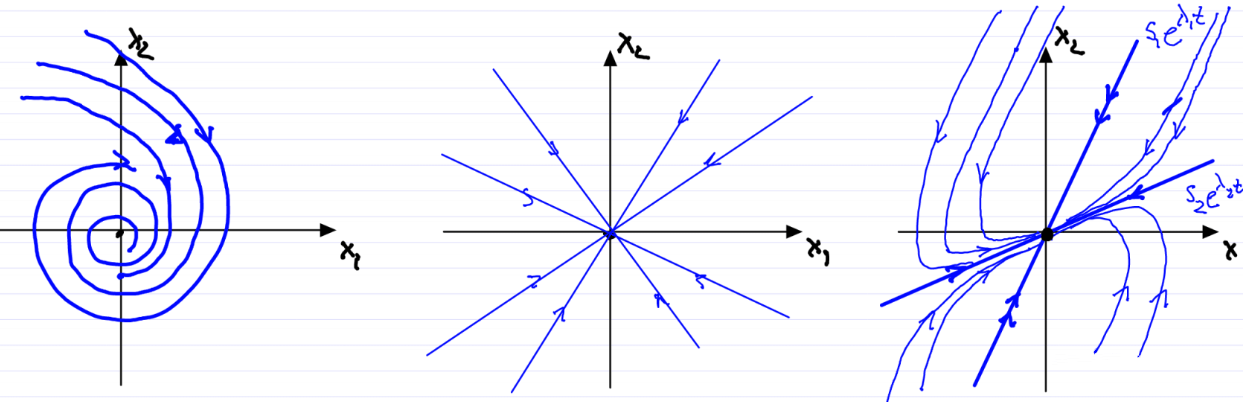
\includegraphics[width=0.9\textwidth]{figures/ch2/13topo_equiv.png}
		\caption{Three topologically equivalent 2-dimensional linear systems. Left: The stable spiral. Middle: The sink. Left: The stable node.}
		\label{fig:topo_equiv}
	\end{figure}

The stable spiral has the eigenvalues $\lambda _{1,2}= \alpha \pm i \beta $ for $\alpha <0$ and $\beta \neq 0$. The sink has the eigenvalues $\lambda_1=\lambda_2<0$. and The stable node has the eigenvalues $\lambda_1 < \lambda_2 < 0$. Note here that the number of eigenvalues $\lambda_i$ with $ \textrm{Re} \lambda_i <0$, $ \textrm{Re} \lambda _i=0$, and $ \textrm{Re} \lambda _i>0$ is the same in all three of these cases, namely for each system the real part of both eigenvalues are less than 0.	
\end{ex}

\begin{remark}[]
	The above systems are not $\mathcal{C}^k$ equivalent or conjugate, as the spectra differ by more than a multiplicative constant.
\end{remark}


\begin{ex}[Topologically inequivalent linear systems for $n=2$]
	As a counter example, we now present three linear systems which are not topologically equivalent. The stable spiral (from before), the unstable spiral, and the saddle. The unstable spiral has the eigenvalues $\lambda _{1,2}= \alpha \pm i \beta $ for $\alpha > 0$ and $\beta \neq 0$ (note the different sign for $\alpha)$. The saddle has the eigenvalues $\lambda _1 < 0 < \lambda_2$. These systems are depicted in Fig \ref{fig:topo_inequiv}.
	\begin{figure}[h!]
		\centering
		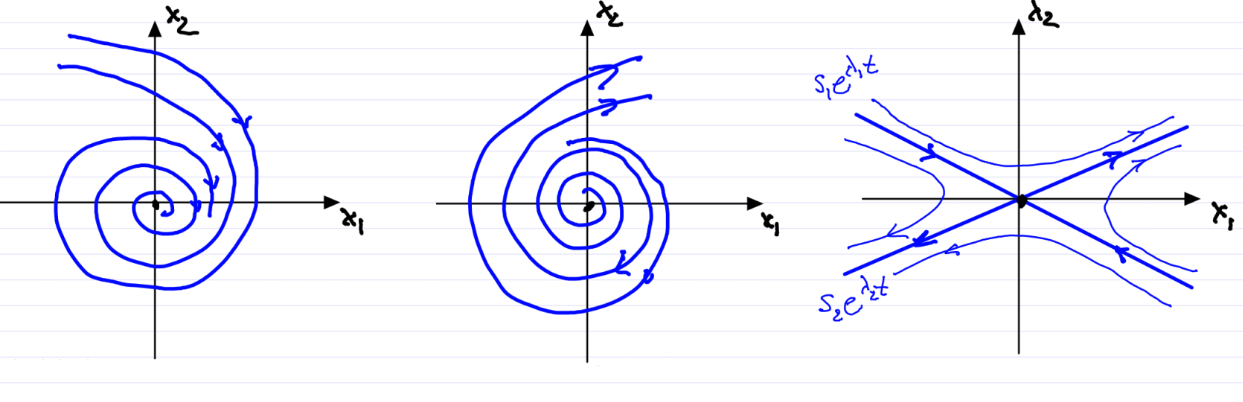
\includegraphics[width=0.9\textwidth]{figures/ch2/14topo_inequiv.png}
		\caption{Three 2-dimensional linear systems which are not topologically equivalent. Left: The stable spiral. Middle: The unstable spiral. Right: The saddle.}
		\label{fig:topo_inequiv}
	\end{figure}

	Note here that the eigenvalue configurations in terms of the number of $\lambda _i$ with real part less than $0$ are different in each case.
Building on the role of the eigenvalue configuration we noted in the previous examples, we introduce the concept of a hyperbolic fixed point.
\end{ex}
\begin{definition}[Hyperbolic fixed point]
	We call the fixed point  ${x} ={x_0} $ a \emph{hyperbolic fixed point} of \eqref{eq:unostar} if each of the eigenvalues $\lambda_i$ of its linearization \eqref{eq:dosstar} satisfy
	\begin{align}
		\boxed{ \textrm{Re} \lambda_i \neq 0.}
	\end{align}
	Geometrically the eigenvalue configuration of a hyperbolic fixed point is shown in Fig. \ref{fig:hyperbol_ex}.
	\begin{figure}[h!]
		\centering
		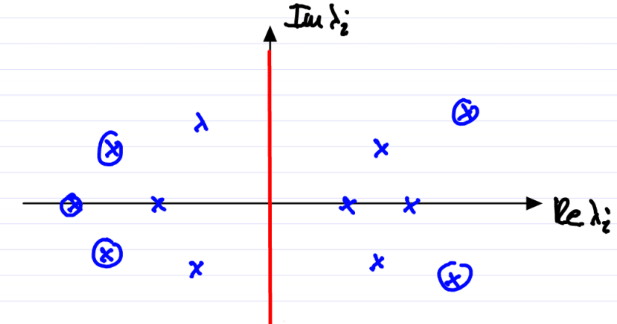
\includegraphics[width=0.6\textwidth]{figures/ch2/15hyperbol_ex}
		\caption{The eigenvalue configuration of a hyperbolic fixed point, i.e. no eigenvalues are on the imaginary axis (red).}
		\label{fig:hyperbol_ex}
	\end{figure}
\end{definition}
	
\begin{proposition}[]
	Under small perturbations to the nonlinear system, the linearized stability type of the hyperbolic fixed point is preserved.
\end{proposition}
Before proving this result, recall the Implicit Function Theorem (without proof).

\begin{theorem}[Implicit Function Theorem ($n+1$ dimensional case)]
	For a function $F:\mathbb{R}^{n+1} \to \mathbb{R}^{n}$ which is $\mathcal{C}^1$, if  $F( {x_0} , y_0 ) = 0$ and the Jacobian $D_{{x} }F({x_0} , y_0 )$ is nonsingular (invertible), then there exists a nearby solution to $F({x} , y )=0 $, for ${x_y} = {x_0}  + \mathcal{O}(|y-y_0|)$. Further ${x_y} $ is as smooth in $y$ as $F({x} ,y)$.
\end{theorem}

\begin{proof}[Proof (Proposition)]
	Add a small perturbation to \eqref{eq:uno} i.e.
\begin{align}
	\dot{{x} } = f({x}) + \varepsilon g({x} );\quad |\varepsilon | \ll 1,\quad f({x} _0) =0.
\end{align}
Now we ask if the perturbed system has a fixed point ${x} _{\varepsilon}$ near ${x} _0$. We frame this in terms of the implicit function theorem
\begin{align}
	F({x} ,\varepsilon) = f({x} ) + \varepsilon g({x} ) \stackrel{?}{=} 0;\quad F({x}_0, 0) = 0;\quad {x} \in \mathbb{R}^{n}, \quad F:\mathbb{R}^{n+1} \to \mathbb{R}^{1}.
\end{align}
We check that $D_{{x} }F({x_0} ,0) $ is nonsingular exactly when $Df({x_0)} $ is; this is fulfilled as we have no zero eigenvalues. The linearization at the perturbed fixed point takes the form
\begin{align}
	\dot{{y} } = D \left. \left[ f({x} ) + \varepsilon g({x} ) \right]\right|_{{x} = {x_\varepsilon} }{y} = \left[ Df({x_0}  + \mathcal{O}(\varepsilon)) + \varepsilon Dg({x_0} + \mathcal{O}(\varepsilon)) \right] {y} 
		=\underbrace{ \left[ Df({x_0})+ \mathcal{O}(\varepsilon) \right]}_{={A_{\varepsilon}} }{y}.
\end{align}
In the last equality we used the Taylor expansion in $\varepsilon$. We have that the roots of $\det({A_{\varepsilon}}-\lambda {I} ) = 0 $ depend continuously on the parameter $\varepsilon$. These roots correspond to the eigenvalues of $A_{\varepsilon}$. Therefore, the roots stay within an $\mathcal{O}(\varepsilon)$ neighborhood of the eigenvalues of $Df({x_0} )$ (see Fig. \ref{fig:eps_ball_eigv}). Hence we have that the eigenvalue configuration is unchanged for small enough $\varepsilon$.
\begin{figure}[h!]
	\centering
	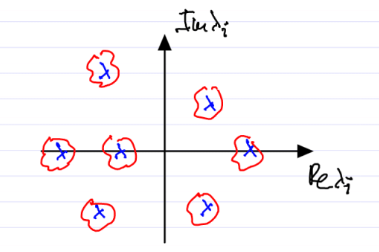
\includegraphics[width=0.5\textwidth]{figures/ch2/16eps_ball_eigv.png}
	\caption{The eigenvalue configuration the $\mathcal{O}(\varepsilon)$ neighborhood (red) drawn around each eigenvalue (blue).}
	\label{fig:eps_ball_eigv}
\end{figure}
\end{proof}
\begin{remark}[]
	In the above proof, not only does the hyperbolicity of fixed points remain preserved, but also the stability type.
\end{remark}
Meanwhile, for nonhyperbolic fixed points, this is not the case, and the smallest perturbation may change their stability type. This is due to the fact, that no matter how small the scale of the perturbation ($\varepsilon$) the $\mathcal{O}(\varepsilon)$ ball around eigenvalues on the imaginary axis will always intersect with $\mathbb{C}- \{  \textrm{Im}\lambda_i =0 \}$ (i.e. points which are not on the imaginary axis).

Now we would like to connect the preservation of stability type under nonlinear perturbation to analyzing the stability type of fixed points of nonlinear dynamical systems based on their linearization. 
\begin{theorem}[Hartman-Grobman]
	If the fixed point ${x_0} $ of the nonlinear system \eqref{eq:unostar} is hyperbolic, then the linearization \eqref{eq:dosstar} is topologically equivalent to the nonlinear system in a neighborhood of ${x_0} $. 

	\textbf{Consequence:} For hyperbolic fixed points, linearization predicts the correct stability type \underline{and} orbit geometry near ${x_0} $. 
\end{theorem}
Now we would like to apply this to the pendulum to systematically derive the stability type of its fixed points.
\begin{ex}[Stability analysis of the pendulum via Hartman-Grobman]
	Recall the transformed ODE for the pendulum
	\begin{align}
		\dot{x}=f(x)=
		\begin{dcases}
		\dot{x}_{1} = x_2 \\ \dot{x}_2 = -\sin(x_1)	
		\end{dcases}
		;\quad {x}  = 
		\begin{pmatrix}
			x_1 \\ x_2
		\end{pmatrix}
		.
	\end{align}
	We have two fixed points ${p} =(\pi ,0)$ and ${q} = (0,0)$. First we analyze the stability of the fixed point ${p} $. The differential of $f$ at a point $a$ is
\begin{align}
	Df(a) =  
		\begin{pmatrix}
			0 & 1 \\
			-\cos(a_1) & 0
		\end{pmatrix}.
\end{align}
	Start by linearizing at ${p} $ 
	\begin{align}
		\dot{{y} } = {Ay};\quad {A}  = Df({p} ) = 
		\begin{pmatrix}
			0 & 1 \\
			- \cos(x_1) & 0
		\end{pmatrix}_{{x} = {p} } =
		\begin{pmatrix}
			0 & 1 \\ 1 & 0
		\end{pmatrix}.
	\end{align}
	Now we have to check if ${p} $ is hyperbolic
	\begin{align}
		\det({A} - \lambda {I} ) = \lambda^2 -1 = 0 \implies \lambda_{1,2} = \pm 1;\ {s_1} =
		\begin{pmatrix}
			1 \\ 1
		\end{pmatrix}
		,\ {s_2} =
		\begin{pmatrix}
			-1 \\ 1
		\end{pmatrix}.
	\end{align}
	Neither of the eigenvalues lie on the imaginary axis, so $p$ is hyperbolic. This allows us to move between the nonlinear and linearized system for the stability analysis without compromising our results. We find the linearized dynamics to be
	\begin{align}
		{y} (t) = C_1 e^{t} {s_1}  + C_2 e^{-t}{s_2}.
	\end{align}
	Using the initial conditions $y_0$ the trajectory can be expressed as
	\begin{align}
		y(t) =  F^{t}{y_0}, 
	\end{align}
	where $F^{t}$ is the normalized fundamental matrix solution. We can now fully describe the phase portrait of the linearization. The \emph{stable subspace} $E^{S}$ is $ \textrm{span} \{{s_2} \} = \{{y_0} :\ F^{t}{y_0} \xrightarrow{t \to \infty} 0 \} $. The unstable subspace $E^{U}$ is $ \textrm{span} \{{s_1}\} = \{{y_0} : \ F^{t}{y_0} \xrightarrow{t \to - \infty }0\} $. The phase portrait near the fixed point $p$ is illustrated in Fig. \ref{fig:pend_phase_p}
\begin{figure}[h!]
	\centering
	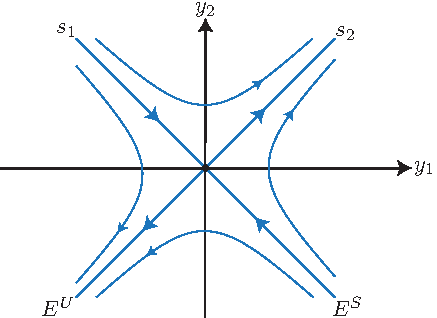
\includegraphics[width=0.4\textwidth]{figures/ch2/17pend_phase_p}
	\caption{The phase portrait of the linearized pendulum in a neighborhood around ${p} $.}
	\label{fig:pend_phase_p}
\end{figure}

The nonlinear phase portrait is topologically equivalent to the linear one. Further we can define the stable and unstable manifolds of ${p} $ for the nonlinear system. We designate $F^{t}(\cdot)$ to be the flow map for the nonlinear system after this point.
The \emph{stable manifold} of ${p} $ is 
\begin{align}
	\boxed{
	W^{S} = \{ {x_0} :\ F^{t}({x_0} ) \xrightarrow{t \to \infty}{p} \}.
}
\end{align}
and the \emph{unstable manifold} of ${p} $
\begin{align}
	\boxed{
	W^{U}=\{{x_0} :\ F^{t}({x_0} ) \xrightarrow{t \to - \infty}{p}\}.
}
\end{align}
Both of these are $\mathcal{C}^{0}$ curves through ${p}$ and their existence follows from the Hartman-Grobman theorem. These manifolds are shown in the nonlinear phase portrait around ${p} $ in Fig. \ref{fig:nonlin_pend_phase_p}. 
\begin{figure}[h!]
	\centering
	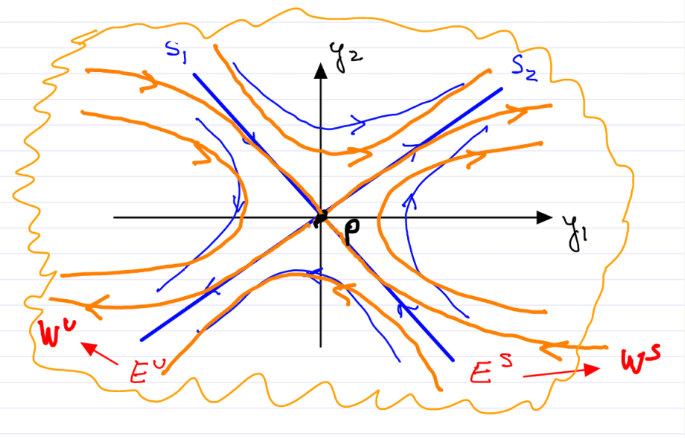
\includegraphics[width=0.6\textwidth]{figures/ch2/18nonlin_pend_phase_p.png}
	\caption{The phase portrait of the pendulum on a neighborhood around ${p} $ with the stable and unstable manifolds of the nonlinear system as well as the stable and unstable spaces of the linearization.}
	\label{fig:nonlin_pend_phase_p}
\end{figure}

Next we analyze the stability of the fixed point $q$. Once again, our first step is to linearize
\begin{align}
	\dot{y} = Ay, \quad A = Df(q) = 
	\begin{pmatrix}
		0 & 1 \\ -1 & 0
	\end{pmatrix}
	;\quad \det (A- \lambda I) = 0.
\end{align}
From here, we see that the determinant is equal $\lambda^2 + 1 = 0$, yielding the roots $\lambda_{1,2}= \pm i$, i.e. the fixed point is \underline{not} hyperbolic. Thus the linearized dynamics is inconclusive for the nonlinear system. In this particular case, $q$ turns out to be stable by the definition of Lyapunov stability. Later we will use another approach to show this directly.
\end{ex}

In the last example, the importance of hyperbolicity was not accentuated, as the latter fixed point had the same stability type in the linearized system as in the full system. This leads us to question if there are cases where the stability type between the linear and nonlinear systems is not preserved.

\begin{ex}[Criticality of hyperbolicity in Hartman-Grobman]
	Let the dynamical system be
	\begin{align}
		\dot{x} = ax^3,\quad x\in\mathbb{R},\quad a \neq 0.
	\end{align}
	This system has a fixed point at $x=0$, linearizing here gives
	\begin{align}
		A = \left. 3ax^2 \right|_{x=0} = 0 \implies \dot{y}= 0y = 0.
	\end{align}
	We have a single root $\lambda_1 = 0$, hence $x=0$ is a nonhyperbolic fixed point. Disregarding this fact, we may be inclined to conclude that $x=0$ is a stable fixed point, since $y=0$ is trivially a fixed point of the linearization $\dot{y}=0$. This is not the case, as we can see by analyzing the full nonlinear dynamics for $a>0$ as in Fig. \ref{fig:hyperbol_counter_ex}, where we observe that $x=0$ is an unstable fixed point.
\begin{figure}[h!]
	\centering
	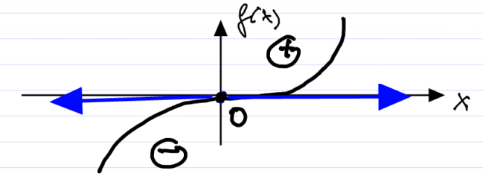
\includegraphics[width=0.5\textwidth]{figures/ch2/19hyperbol_counter_ex.png}
	\caption{Nonlinear dynamics for the dynamical system $\dot{x}= ax^3$ with $a>0$.}
	\label{fig:hyperbol_counter_ex}
\end{figure}
\end{ex}

Now that we have understood how to use the Hartman-Grobman theorem, we would like to to be able to definitely conclude the stability type of a fixed point, once we have the linearization. To achieve this, we require a sufficient and necessary criterion for all of the eigenvalues of the linearized system to be left of the imaginary axis, i.e. $ \textrm{Re} \lambda_i < 0$ for all $i$.

\begin{theorem}[Routh-Hurwitz]
Consider the polynomial
\begin{align}
	a_n \lambda^{n} + a_{n-1} \lambda ^{n-1} + \ldots + a_{1} \lambda + a_0 = 0.
\end{align}
Without loss of generality assume $a_0 > 0$, if $a_0 <0$ then multiply by $-1$ and if $a_0=0$ then $\lambda =0$ is a root and therefore we cannot have asymptotic stability. Next, define the following series of subdeterminants
\begin{align}
	D_0 = a_0,\ D_1 =a_1,\ D_2 =
	\begin{vmatrix}
		a_1 & a_0 \\
		a_3 & a_2
	\end{vmatrix}
	,\ D_3 = 
	\begin{vmatrix}
		a_1 & a_0 & 0 \\
		a_3 & a_2 & a_1 \\
		a_5 & a_4 & a_3
	\end{vmatrix}
	,\ldots,\ D_n =
	\begin{vmatrix}
		a_1 & a_0 & 0 & \ldots & 0 \\
		a_3 & a_2 & a_1 & \ldots & 0 \\
		\vdots & & & & \vdots \\
		0 & \ldots &  a_n & a_{n-1} & a_{n-2}\\
		0 &  \ldots  & & 0  & a_n
	\end{vmatrix}
\end{align}
Then we have that if and only if for all $i$ $D_i >0$ then $ \textrm{Re} \lambda_i <0$ for all $i$.

A weaker neccesary condition is that if for all $i$ $ \textrm{Re} \lambda _i<0$ then $a_i >0$ for all $i$. Therefore if there exists an $a_k<0$, we know immediately that the fixed point cannot be asymptotically stable as not all of the $ \textrm{Re} \lambda _i $ can be strictly negative.
\end{theorem}
\begin{remark}[]
For a given $i$ we construct the matrix used for calculating $D_i$ as follows: write the elements $a_1,\ldots,a_i$ along the diagonal, then in each row $k$ write the $a_j$ in descending index order such that $a_k$ aligns with the placement inherited from us writing along the diagonal. The leftover spaces are filled with zeros. 
\end{remark}

\begin{remark}[]
	Adolf Hurwitz discovered this criterion independently of Edward Routh in 1895 while holding a chair at the ETH.
\end{remark}

\begin{ex}[Applying the Routh-Hurwitz criterion]
	Given the polynomial
	\begin{align}
		a_3 \lambda ^3 + a_2 \lambda^2 + a_1 \lambda + a_0 = 0.
	\end{align}
	The Routh-Hurwitz criterion is
	\begin{align}
	D_0 = a_0 > 0;\ D_1 = a_1 >0;\ D_2 = a_1 a_2 - a_0 a_3>0;\ D_3 = a_3 D_2 >0.	
	\end{align}
	Therefore 
	\begin{align}
		\boxed{
			a_0> 0,\ a_1 > 0,\ a_1a_2 - a_0a_3 > 0,\ a_3 > 0
		}
	\end{align}
	forms a sufficient and necessary condition for asymptotic stability ($a_i >0$ follows from here) for $n=3$.
\end{ex}

A more refined linearization result comes from Sternberg's Theorem \cite{Chicone}.
\begin{theorem}[Sternberg]
Assume the following
\begin{enumerate}
	\item The fixed point is asymptotically stable, i.e. $ \textrm{Re} \lambda _j<0$ for all $j=1,\ldots,n$ (this also implies hyperbolicity);
	\item $f\in \mathcal{C}^{r}$ for $r\in \mathbb{N}\cup \{\infty \}$ and $r>\frac{\max_{j}| \textrm{Re} \lambda _j|}{\min_{j}| \textrm{Im} \lambda _j|}$;
	\item The system is nonresonant, i.e. 
		\begin{align}
			\sum_{j=1}^{n}m_j \lambda _j \neq \lambda_k,\ \forall k
		\end{align}
	for any sequence $m_j \in \mathbb{N}$ with $\sum_{j=1}^{n} m_j \geq 2$.
	
\end{enumerate}
Then the following holds: $\dot{x}=f(x)$ with $f(0)=0$ is locally $\mathcal{C}^{r}$ conjugate to its linear part $\dot{y}=Ay$ for $A= Df(0)$.
\end{theorem}


\begin{ex}[Watt's centrifugal governor for steam engines]
	Now we put together everything built until now in the example of Watt's centrifugal governor for steam engines. Originally this system was used in mills in the 1700's, then it was adapted by Watt to the steam engine in 1788. This adaptation has been credited as a major factor in the industrial revolution, and is a first example of feedback control. The system is outlined in Fig. \ref{fig:governor}.
\begin{figure}[h!]
	\centering
	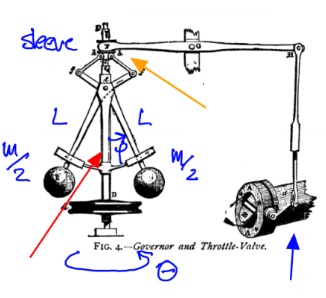
\includegraphics[width=0.34\textwidth]{figures/ch2/20governor.png}
	\caption{Schematic for Watt's centrifugal governor. The yellow arrow points towards a damper on the rotation about the spindle (red arrow). On the right the blue arrow designates a steam engine cylinder.}
	\label{fig:governor}
\end{figure}
The two masses (of mass $\frac{m}{2}$) rotate counter clockwise, and their position in radians is given by $\theta$, with their rotational velocity $\dot{\theta}$. The masses are attached by a rod of length $L$ and their deflection from the vertical position is measured by $\varphi$. Smaller $\dot{\theta}$ allowed for an increase in steam supply.

Following changes in the design, the systems suddenly became unstable. To address this Vyshnegradsky studied the root cause in 1877. We first derive the equation of motion. For the governor we use the equation of motion for a rotating hoop (with viscous damping coefficient $b$).
\begin{align}
	mL^2 \ddot{\varphi} + bL^2\left( \frac{g}{L} - \dot{\theta}^2 \cos(\varphi) \right) \sin(\varphi) = 0;\quad b>0.
\end{align}
Next, let $\omega $ denote the angular velocity of the steam engine, i.e. with the gear ratio $n$ we have $\dot{\theta} = n \omega$. Then we find
\begin{align}
	m \ddot{\varphi} = -b \dot{\varphi} - m \left( \frac{g}{L} - n^2 w^2 \cos(\varphi) \right) \sin(\varphi).
\end{align}
Now we derive the equation of motion for the steam engine. Denote the moment of inertia for the engine by $J$, the driving torque from the steam as $P_1$ and the constant load $P$, we obtain
\begin{align}
	J \dot{\omega } = P_1 - P.
\end{align}
In this case we have $P_1 = P^{*} + k\left( \cos(\varphi) - \cos(\varphi^{*}) \right)$ for the desired operation angle $\varphi^{*}$, the gain $k$, and $P*$ the value of $P$ at $\varphi^{*}$. Putting this together yields
\begin{align}
	J \dot{\omega } = k \cos(\varphi) - P_0;\quad P_0 = P - P^{*} + k \cos(\varphi^{*}).
\end{align}
Let $\dot{\varphi} = \Psi$ to transform into a three-dimensional set of equations (ODE)
\begin{align}
	\begin{dcases}
		\dot{\varphi} = \Psi \\
		\dot{\Psi} = -\frac{b}{m} \Psi - \left( \frac{g}{L} - n^2 \omega^2 \cos(\varphi) \right) \sin (\varphi) \\
		\dot{\omega } = \frac{k}{J}\cos(\varphi) - \frac{P_0}{J}.
	\end{dcases};
	\quad x =
	\begin{pmatrix}
		\varphi \\ \Psi \\ \omega 
	\end{pmatrix}
	.
\end{align}
Then our operation point is the fixed point $x_0$ of this system
\begin{align}
	f(x_0) = 0 \implies \Psi_0 = 0;\ \omega_0^2 = \frac{g}{Ln^2 \cos(\varphi_0)};\ \cos(\varphi_0) = \frac{P_0}{k}.
\end{align}
If $\sin(\varphi_0)=0$, we have an unphysical state and ignore this case. For simplification set $L=1$, this could be formally achieved by nondimensionalizing the length $L$. Now we linearize at the fixed point $x_0$ 
\begin{align}
	\dot{y} = Ay; \quad A = Df(x_0) =
	\begin{pmatrix}
		0 & 1 & 0 \\
		n^2 \omega^2 \cos(2\varphi_0) -g\cos(\varphi_0) & -\frac{b}{m} & n^2 \omega _0 \sin(2\varphi_0) \\
		-\frac{k}{J}\sin(\varphi_0) & 0 & 0
	\end{pmatrix}
.	
\end{align}
With this we obtain the characteristic equation $\det(A - \lambda I )= 0$ 
\begin{align}
	\underbrace{1}_{a_3} \lambda^3 + \underbrace{\frac{b}{m}}_{a_2}\lambda ^2 + \underbrace{ {g}\frac{\sin^2(\varphi_0)}{\cos(\varphi_0)}}_{a_1} \lambda + \underbrace{ {g} \frac{2k \sin^2 (\varphi_0)}{J \omega_0}}_{a_0} = 0.
\end{align}
Now check the Routh-Hurwitz criterion for asymptotic stability:
\begin{enumerate}
	\item The necessary condition for $ \textrm{Re} \lambda _k<0$ for all $k$: $a_j> 0$ for all $ j$ is fulfilled.
	\item Next we check the subdeterminants
		\begin{subequations}
\begin{align}
	D_0 &= a_0 = {g} \frac{2k \sin^2 (\varphi_0)}{J \omega_0}>0;\quad \\ 
	D_1 &= a_1 = {g}\frac{\sin^2 (\varphi_0)}{\cos(\varphi_0)} >0; \\
	D_2 &= 
	\begin{vmatrix}
		a_1 & a_0 \\
		a_3 & a_2
	\end{vmatrix}
	= a_1a_2 - a_0a_3 = g\frac{b}{m}\frac{\sin^2(\varphi_0)}{\cos(\varphi_0)} - g\frac{2k \sin^2(\varphi_0)}{J \omega_0} >0;\\
	D_3 &> 0 \iff D_2 >0  \textrm{ and } a_3=1>0.
\end{align}
		\end{subequations}
The only actual condition for $x_0$ to be asymptotically stable is $D_2 >0$ 
\begin{align}
	\frac{bJ}{m} > \frac{2 P_0}{\omega_0}.
\end{align}
From the equation for the fixed points we know 
\begin{subequations}
\begin{align}
	P_0 \omega_0^2 = \frac{gk}{n^2} =  \textrm{const.} \numberthis \label{eq:watt1}\\
	\omega_0^2 + 2P_0 \omega_0 \frac{d \omega_0}{d P_0} = 0.
\end{align}
\end{subequations}
From the first equation, we realize that we must write $\omega_0 = \omega_0(P_0)$. To obtain the second equation, we derive the first equation \eqref{eq:watt1} with respect to $P_0$. Therefore we find 
\begin{align}
	\frac{d \omega_0}{d P_0} = - \frac{\omega_0}{2P_0}.
\end{align}

\end{enumerate}
Next, define the \emph{non-uniformity of performance}
\begin{align}
	\nu = \left| \frac{d \omega_0}{d P_0} \right| = \frac{\omega_0}{2P_0}.
\end{align}
Then our criterion for asymptotic stability becomes
\begin{align}
\frac{bJ}{m}\nu > 1.	
\end{align}
To conclude, the following have harmful effects of stability
\begin{itemize}
	\item Bigger engines which increase $m$ 
	\item Better machining of surfaces decreasing $b$ 
	\item Increased operating speed decreasing $J$ 
	\item Versatility in operation decreasing $\nu $.
\end{itemize}
These have the effect of pushing the eigenvalues to the right in the complex plane (towards the imaginary axis) as is illustrated in Fig \ref{fig:watt_eigv}.
\begin{figure}[h!]
	\centering
	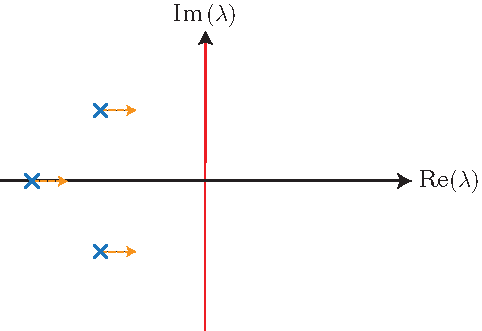
\includegraphics[width=0.4\textwidth]{figures/ch2/21watt_eigv}
	\caption{Change in the eigenvalue configuration as small modification are made to the Watt engine governor.}
	\label{fig:watt_eigv}
\end{figure}
\end{ex}
\newpage

 \section{Data-driven linear modeling of dynamical systems}
 Given are $m+1$ vectors of $n$-dimensional observables $x_0,\ldots,x_m \in \mathbb{R}^{n}$ observed at $\Delta t$ intervals. An example of such data would be many different trajectories or snapshots of a single trajectory. Typically $m \gg 1$, i.e. there are a high number of observations.

 Our objective is to find the best fitting linear dynamical system
 \begin{align}
 	\dot{x}=Ax;\quad x \in \mathbb{R}^{n};\quad A \in \mathbb{R}^{n\times n}.
 \end{align}
Since the data is given as discrete observations, this is equivalent to seeking the best $B=e^{A\Delta t}$ such that $x_{k+1} =Bx_k$ for $k=1,\ldots, m-1$. To solve this we synthesize the data into matrices
\begin{align}
	X = 
	\begin{bmatrix}
		x_0 \ldots x_{m-1}
	\end{bmatrix}
	\in \mathbb{R}^{n\times m}
;\quad
	Y = 
	\begin{bmatrix}
		x_1 \ldots x_{m}
	\end{bmatrix}
	\in \mathbb{R}^{n\times m}.
\end{align}
Notice that the matrix $Y$ is shifted forward compared to the matrix $X$ by $\Delta t$. Next, we solve for  a matrix $B$ that minimizes the distance between $Y $ and $BX$. That is, we find
\begin{align}
	B_{*} =  \underset{B \in \mathbb{R}^{n\times n}}{\textrm{argmin }} g(B);\quad g(B) = \| Y - BX \|^{2} \numberthis \label{eq3:star},
\end{align}
where the matrix norm is the Frobenius norm. We denote the components of $B$ by $b_{ij}$, the components of $Y$ by $y_{ij}$, and the components of $X$ by $x_{ij}$. Note that
\begin{subequations}
\begin{align}
	\frac{\partial g}{\partial b_{ij}} &= \frac{\partial}{\partial b_{ij}} \sum_{l,m,p}^{} \left(y_{lm} - b_{lp}x_{pm}\right)^{2} 
	= -2 \sum_{l,m,p}^{} \left( y_{lm}-b_{lp}x_{pm}\right) \delta_{il}\delta_{jp}x_{pm} \\
					   &= -2\sum_{m,p}^{} \left(y_{im}-b_{ip}x_{pm}\right) x_{jm} 
					   = 2\left(YX^{T} - BX X^{T}\right).
\end{align}
\end{subequations}
In the third equality we have used the properties of the Kronecker-delta $\delta_{ij}$. Therefore we must have that $D_{B}g = -2\left(YX^{T} - BXX^{T}\right)=0$, so we must solve the linear system of equations
\begin{align}
	BXX^{T} = YX^{T}\in \mathbb{R}^{n \times n}.
\end{align}
In the case $n>m$, the matrix $X^{T}$ has more columns than rows, thus $X^{T}$ is singular. Hence $XX^{T}$ has a nonempty kernel and is therefore not invertible. For $n<m$ this is not necessarily the case. For a solution, we can use the pseudo inverse $(XX^{T})^{\dagger}$, the superscript here is called \emph{dagger}.

Recall that if $A \in \mathbb{R}^{n\times n}$ is invertible then $A^{-1} = A^{\dagger}$. If $A$ is not invertible, then calculate the singular value decomposition of $A = U \Sigma V^{T}$ for $U,V \in  \textrm{SO} (n)$ and $\Sigma$ a diagonal matrix. The entries of $\Sigma$ are the strictly positive singular values. The columns of $U$ and $V$ are the left and right singular vectors. We then define the pseudo inverse as
\begin{align}
	A^{\dagger} = V \Sigma^{\dagger} U^{T};\quad \Sigma_{ij}^{\dagger} = 
	\begin{cases}
		\frac{1}{\Sigma_{ij}} & \Sigma_{ij} \neq 0\\
		0 & \Sigma_{ij}=0.
	\end{cases}
\end{align}

This means that for $Ax=b$, the best solution in a least squares sense is given by $x= A^{\dagger}b$. In our case, the solution to \ref{eq3:star} is 
\begin{align}
	B = \left(Y X^{T}\right) \left( XX^{T}\right)^{\dagger}.
\end{align}
This procedure is called \emph{dynamic mode decomposition} (DMD) \cite{Schmid2010, Kutz2016}. The eigenvectors of $B$ are called \emph{DMD modes} and the normalized exponents of those corresponding eigenvalues are called \emph{DMD eigenvalues}.

The procedure has been extended in \emph{extended DMD}, where DMD was performed on functions of the observables (typically polynomials) \cite{Williams2015}. This effectively tries to construct the linearization from data. Note here that none of these procedures can describe intrinsically nonlinear phenomena (i.e. those with coexisting isolated compact invariant sets). 

\begin{remark}[]
The numerical cost of (pseudo)inverting the $n \times n$ matrix, $XX^T$, can be reduced when $n\gg m$.
\begin{enumerate}
\item We can calculate the singular value decomposition of the data matrix $X$ instead. 
\item By keeping only the leading $r$ singular values in this decomposition, we obtain a reduced (rank-$r$) approximation of the matrix $B\in \mathbb{R}^{n \times n}$ as follows. Denote the singular value decomposition by $X = U\Sigma V^T$.  This also means that $(XX^T) = U\Sigma^2 U^T$, i. e. we get the same $U$ as before, but from an SVD of an $n\times m$ matrix, which is much less demanding numerically.

 With the leading $r$ singular vectors and singular values $\sigma$, $X$ can be written as
\begin{equation}
X \approx U_r \Sigma_r V_r^T = \sum_{i=1}^r \sigma_i u_i v_i^T, \qquad U = [u_1, ..., u_n]\quad V = [v_1, ..., v_m].
\end{equation}
\item The matrix $B$ can be approximately written as 
	\begin{subequations}
\begin{align}
B &= YX^T(XX^T)^\dagger \\
& \approx YV_r\Sigma_rU_r^TU_r(\Sigma_r^2)^\dagger U_r^T \\
&= YV_r\Sigma_r^\dagger U_r^T = Y(X_r)^\dagger.
\end{align}\end{subequations}
We denote the truncated approximation of $B$ as $B_r = Y (X_r)^\dagger.$
\end{enumerate}
\end{remark}
	
	
\section{Lyapunov's direct (second) method for stability}
Stability analysis via linearization is not perfect. For nonhyperbolic fixed points, the results obtained are inconclusive, and this case turns out to be somewhat common for conservative systems. Furthermore, linearization does not give any insight into the size of the domain of stability. Hence, a method for determining stability type without relying on linearization would be desirable. This is given to us by Lyapunov's direct method.

\begin{theorem}[] \label{thm:direct}
	Consider
	\begin{align}
		\dot{x} = f(x), \quad f\in \mathcal{C}^1,\quad x \in \mathbb{R}^{n};\quad f(x_0) = 0.
	\end{align}
	Assume that there exists a function $V:U \to \mathbb{R}$ with $V\in \mathcal{C}^1(U)$ for an open set $U \subset \mathbb{R}^{n}$ and $x_0 \in U$ which fulfills the following
	\begin{enumerate}
		\item $V$ is positive definite in a neighborhood of $x_0$, i.e.
			\begin{align}
				V(x_0)=0;\quad V(x)>0,\ x\in U-\{ x_0 \}.
			\end{align}
		\item $\dot{V}$ is negative semidefinite in the same neighborhood, i.e.
			\begin{align}
				\dot{V} =\frac{d}{dt}V(x(t))= 
				\langle DV(x(t)), \dot{x}(t) \rangle =
				\langle DV(x(t)), f(x(t)) \rangle \leq 0,\ x\in U.
			\end{align}
	\end{enumerate}
	Then $x=x_0$ is Lyapunov stable (cf. Def. \ref{def:stable}). $V$ is called a Lyapunov function. The hypotheses are illustrated in Fig. \ref{fig:lyap_thm_assumptions}.	
\end{theorem}
\begin{figure}[h!]
	\centering
	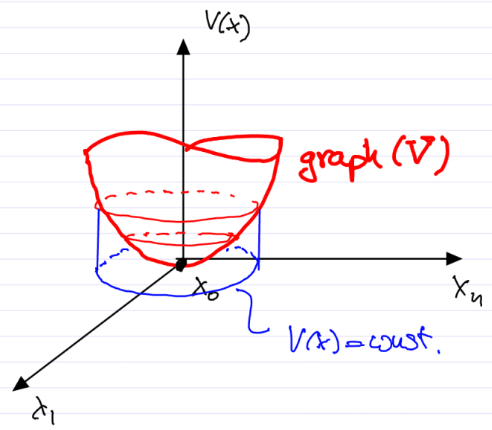
\includegraphics[width=0.4\textwidth]{figures/ch2/23lyap_thm_assumptions1.png}
	\hspace{0.05\textwidth}
	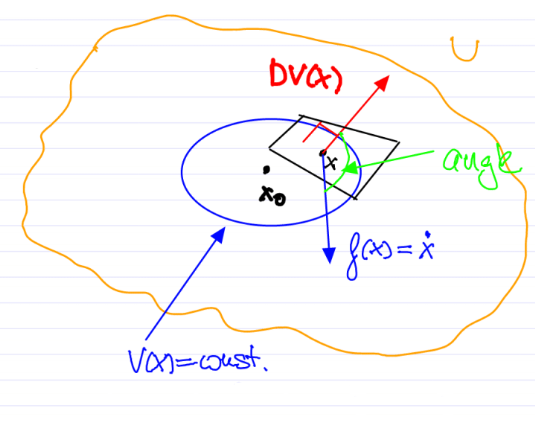
\includegraphics[width=0.4\textwidth]{figures/ch2/23lyap_thm_assumptions2.png}
	\caption{Geometric interpretation of hypotheses of Lyapunov's direct method. Left depicts hypothesis (i) and right hypothesis (ii). The angle between $DV(x)$ and $f(x)$ is at least $\frac{\pi }{2}$. In each image the blue $V(x)=$const. is a level surface diffeomorphic to $S^{n-1}$.}
	\label{fig:lyap_thm_assumptions}
\end{figure}

	\begin{remark}[]
		To denote the boundary of a set $A$ we write $\partial A$.
	\end{remark}
\begin{proof}
	
	First choose $\varepsilon > 0$ and define $\alpha(\varepsilon)= \min_{x\in \partial B_\varepsilon(x_0)} V(x) > 0$. Note that $\alpha(\varepsilon)$ is well defined as $V\in \mathcal{C}^{0}(U)$ and $\partial B_{\varepsilon}(x)$ is compact and spherical for small enough $\varepsilon$. There exists an $x^{*} \in \partial B_{\varepsilon}(x)$ with $V(x^{*}) = \alpha(\varepsilon) \leq V(x)$ for all $x\in \partial B_{\varepsilon}(x_0)$. Next, define $U_{\varepsilon}= \{ x\in B_{\varepsilon}(x_0):\ V(x) < \alpha(\varepsilon)  \ $. Notice that $x_0 \in U_{\varepsilon}$ because $V(x_0) =0$ and $V(x)\geq 0$ on $U$. Further $U_{\varepsilon}$ is open due to the continuity of $V$. We have that  $U_{\varepsilon} \cap \partial B_{\varepsilon}(x_ 0) $ is empty by definintion, noting that for all $x\in \partial B_{\varepsilon}(x_0)$ we have $V(x) \geq \alpha(\varepsilon) $. Therefore there exists a ball $B_{\delta(\varepsilon)} \subset U_{\varepsilon} $ which contains $x_0$. This can be seen in Fig. \ref{fig:lyap_pf_1}.
\begin{figure}[h!]
	\centering
	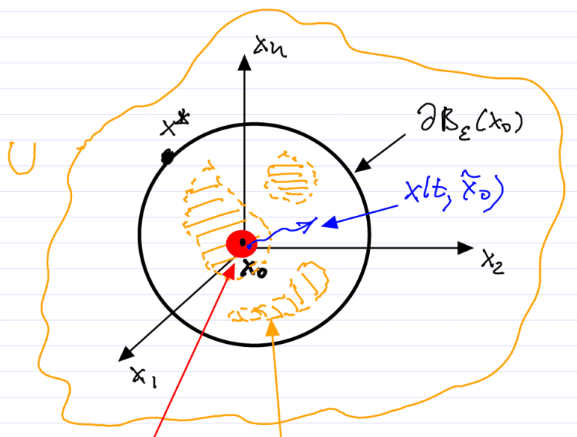
\includegraphics[width=0.45\textwidth]{figures/ch2/22lyap_pf_1.png}
	\caption{The constellation of $U$, $U_\varepsilon$, $\partial B_{\varepsilon}(x_0)$, and $B_{\delta(\varepsilon)}(x_0)$ from the proof of Lyapunov's direct method. The red arrow points at $B_{\delta(\varepsilon)}(x_0)$ and the yellow arrow at a connected component of $U_\varepsilon$.}
	\label{fig:lyap_pf_1}
\end{figure}

Now observe that for every $\tilde{x}_{0} \in B_{\delta(\varepsilon)}(x_0)$ we have that along trajectories $V(x(t; \tilde{x}_{0})) \leq V(\tilde{x}_{0}) < \alpha(\varepsilon)$. The first inequality comes from hypothesis (ii) and the second inequality from the definition of $U_{\varepsilon}$. This implies that for $x(t; \tilde{x}_0) \in U_{\varepsilon}$ we have that $x(t; \tilde{x}_{0})$ is not in $\partial B_{\varepsilon}(x_0)$ for any $t> 0$. The trajectory $x(t; \tilde{x}_0)$ is continuous, in order for it to leave the ball $B_{\varepsilon}(x_0)$ it must intersect the boundary $\partial B_{\varepsilon}(x_0)$. At this point $V(x)$ will atain a value of at least $\alpha(\varepsilon)$ by definition, however this is in contradiction to the fact that $V(x(t;\tilde{x}_0))$ is strictly smaller that $\alpha(\varepsilon)$. Therefore must stay in the ball $B_{\varepsilon}(x_0)$ for all times.
\end{proof}

Now we present some extensions to this theorem for various different stability types. These are necessary, as the previous theorem only provides a sufficient condition for stability (it is not ``if and only if").

\begin{theorem}[Theorem 2]
Consider the same dynamical system. Assume
\begin{enumerate}
	\item $V(x)$ is positive definite,
	\item $\dot{V}(x)$ is negative definite, i.e.
		\begin{align}
			\dot{V}(x) < 0,\ x\in U- \{x_0\}.
		\end{align}
\end{enumerate}
		Then $x=x_0$ is asymptotically stable. These hypotheses are illustrated in Fig. \ref{fig:lyap_thm2_hypos}.
\end{theorem}
\begin{figure}[h!]
	\centering
	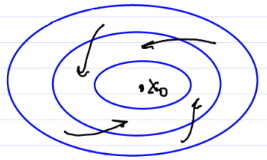
\includegraphics[width=0.4\textwidth]{figures/ch2/24lyap_thm2_hypos.png}
	\caption{The hypotheses of Theorem 2 illustrated, the key difference being that the arrows (denoting the flow of the dynamical system) cross the level surfaces of $V$ (blue rings) toward $x_0$.}
	\label{fig:lyap_thm2_hypos}
\end{figure}

\begin{theorem}[Theorem 3]
	Consider the same dynamical system. Assume
	\begin{enumerate}
		\item $V(x)$ is positive definite,
		\item $\dot{V}(x)$ is positive definite, i.e.
		\begin{align}
			\dot{V}(x)>0,\ x\in U- \{x_0\}.
		\end{align}
	\end{enumerate}
	Then $x=x_0$ is unstable. The hypotheses are illustrated in Fig. \ref{fig:lyap_thm3_hypos}.
\end{theorem}

\begin{figure}[h!]
	\centering
	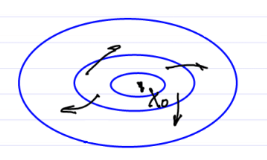
\includegraphics[width=0.4\textwidth]{figures/ch2/25lyap_thm3_hypos.png}
	\caption{The hypotheses of Theorem 3 illustrated, the key difference being that the arrows (denoting the flow of the dynamical system) cross the level surfaces of $V$ (blue rings) away from $x_0$.}
	\label{fig:lyap_thm3_hypos}
\end{figure}

\begin{theorem}[Theorem 4]
	Consider the same dynamical system. Assume
	\begin{enumerate}
		\item $V(x)$ is indefinite, i.e. arbitrarily close to $x_0$ there exists $a,b \in U$ such that $V(x_1)\cdot V(x_2) <0$ (they have opposite signs and are not equal to 0) and $V(x_0)=0$. Furthermore, this is a critical point, i.e. $DV(x_0)=0$.
		\item $\dot{V}(x)$ is definite near $x_0$ (either positive or negative).
	\end{enumerate}
	Then $x=x_0$ is unstable. The geometry of the hypotheses are  illustrated in Fig. \ref{fig:lyap_thm4_hypos}.
\end{theorem}

\begin{figure}[h!]
	\centering
	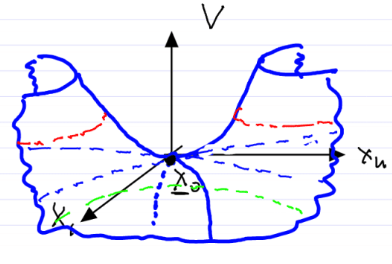
\includegraphics[width=0.4\textwidth]{figures/ch2/26lyap_thm4_hypos.png}
	\hspace{0.05\textwidth}
	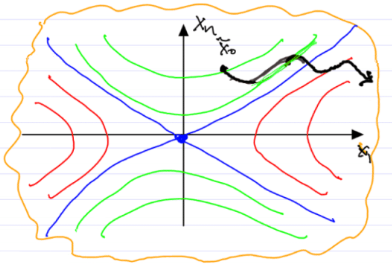
\includegraphics[width=0.4\textwidth]{figures/ch2/26lyap_thm4_hypos2.png}
	\caption{The geometry of hypotheses (i) (left) and (ii) (right) for $\dot{V}$ positive definite of Theorem 4 illustrated. On the right level surfaces are designated by lines, blue corresponds to $V=0$, red $V>0$, and green $V<0$, which can be seen as the dotted lines of the same colors on the left.}
	\label{fig:lyap_thm4_hypos}
\end{figure}

\begin{remark}[]
	In each of these theorems, the definiteness of $ \dot{V}$ can be replaced by semidefiniteness, if we add that the set $\{x\in U:\ \dot{V}(x)=0 \}$ does not contain full trajectories of the system. This is called Krasovsky's condition.
\end{remark}

Now we would like to put these theorems into practice with a few examples.
\begin{ex}[Stability analysis of the pendulum with Lyapunov's direct method]
	Recall that using linearization, we were only able to conclude the stability type of one of the fixed points for the dynamical system of the pendulum
	\begin{align}
		ml^2 \ddot{\varphi} + mgl \sin(\varphi) =0.
	\end{align}
Now we will use the energy as a Lyapunov function, which is often very useful. The energy is given by
\begin{align}
	E(x) = E(\varphi, \dot{\varphi}) = \frac{1}{2}ml^2 \dot{\varphi}^2 + mgl(1-\cos(\varphi)) 
	= \frac{1}{2}ml^2 \dot{x_2}^2 + mgl(1-\cos(x_1)).
\end{align}
Transforming the dynamical system to be an system of first order ODEs we obtain
\begin{align}
	x = 
	\begin{pmatrix}
		x_1 \\x_2
	\end{pmatrix}
	=
	\begin{pmatrix}
		\varphi \\ \dot{\varphi}
	\end{pmatrix}
	;\quad \dot{x}=
	\begin{pmatrix}
		\dot{x_1} \\ \dot{x_2}
	\end{pmatrix}
	=
	\begin{pmatrix}
		x_2 \\ - \frac{g}{l} \sin (x_1)
	\end{pmatrix}
	=f(x).
\end{align}
At the fixed point $x=(0,0)$ we have
\begin{align}
	E(0,0) = 0;\quad DE(0,0) = 0\in \mathbb{R}^{2\times 2};\quad D^2E(0,0) =
\begin{pmatrix}
	mgl & 0 \\
	0 & ml^2
\end{pmatrix}.
\end{align}
We have that the Hessian of $E$ is positive definite. Therefore $E$ is positive definite at $(0,0)$. Further we have
\begin{align}
	\dot{E}(x) = \langle DE(x), f(x) \rangle 
	=
	\begin{pmatrix}
		mgl \sin(x_1) &  ml^2 x_2
	\end{pmatrix}
	\begin{pmatrix}
		x_2 \\ - \frac{g}{l}\sin (x_1)			
	\end{pmatrix}
	= 0.	
\end{align}
Thus $\dot{E}$ is negative semidefinite. Now the hypotheses of Theorem \ref{thm:direct} are fulfilled, hence $x=(0,0)$ is Lyapunov stable. Importantly, this is a nonlinear result and we did not need to refer to the linearization of the system!

At the fixed point $x = (\pi, 0)$. We check again using the energy. First we realize that $E(\pi, 0)= 2mgl$, so we subtract the constant and redefine to obtain $\tilde{E}= E - 2mgl$. Now $\tilde{E}(\pi, 0) = 0$, although this is not essential. Next we calculate
\begin{align}
	DE(\pi, 0) = 0\in \mathbb{R}^{n\times n};\quad D^2E(\pi, 0) = 
	\begin{pmatrix}
		-mgl & 0 \\
		0 & ml^2
	\end{pmatrix}
	.
\end{align}
Hence, $E$ is indefinite at $(\pi, 0)$. From the previous calcuation we alread know that $\dot{E}(\pi, 0) = 0$, i.e. $\dot{E}$ is semidefinite. We cannot apply Theorem 4, but linearization already concluded that $(\pi,0)$ was unstable.

If we add damping the dynamics becomes
\begin{align}
	m\ell^2 \ddot{\varphi} + c \dot{\varphi} mg\ell \sin(\varphi) =0.
\end{align}
Again we transform the system by introducing the coordinates $x_1 =\varphi$ and $x_2=\dot{\varphi}$. Thus we have a first order ODE
\begin{align}
	\begin{dcases}
		\dot{x_1} = x_2 \\
		\dot{x_2} = - \frac{c}{m\ell^2}x_2 - \frac{g}{\ell}\sin(x_1).
	\end{dcases}
\end{align}
We still have the fixed points $(0,0)$ and $(0, \pi)$ and the energy $E = \frac{1}{2}m \ell^2 \dot{\varphi}^2 + mg \ell(1 - \cos(\varphi))$. Again we find
\begin{align}
	DE =
	\begin{pmatrix}
		mg\ell \sin(x_1) \\ m \ell^2 x_2
	\end{pmatrix}
	\implies DE(0) = 0;\quad
	D^2E =
	\begin{pmatrix}
		mg\ell \cos(x_1) & 0 \\
		0 & m \ell^2
	\end{pmatrix}
	.
\end{align}
Thus $E$ is positive definite at $(0,0)$ and indefinite at $(0, \pi )$. We have
\begin{align}
	\dot{E} = DE \cdot f = mgl \sin(x_1)x_2 + m\ell^2 x_2 \left(-\frac{c}{m\ell^2}x^2 - \frac{g}{\ell}\sin(x_1)\right) = - cx_2^2.
\end{align}
Note here that $\dot{E}= -cx_2^2$ is only negative semi-definite. Therefore the asymptotic stability of $x=(0,0)$ and the instability of $x=(0,\pi )$ do not follow from theorems 1 or 4. However, the set $S=\left\{x:\ \dot{E}(x)=0\right\} - \left\{(0,0),\ (0,\pi )\right\}$ does \underline{not} contain full trajectories. Indeed
\begin{align}
	\left.\frac{d}{dt}x_2(t)\right|_{x=0} = -\frac{g}{\ell}\sin(x_1) \neq 0,\ x\in S.
\end{align}
Hence, the asymptotic stability of $(0,0)$ and instability of $(0,\pi )$ follows by Krasovsky's condition.
\end{ex}
 \begin{ex}[Stability analysis of the friction pendulum]
	 We have a shaft which is constantly rotating with angular speed $\Omega $, around this shaft is a sleeve which rubs against the shaft creating friction. To this sleeve is a mass $m$ attached at distance $l$, the deflection of this mass from its standard position (directly below the shaft) is measured by $\varphi$. The gravity constant is given by $g$. This setup is depicted in Fig. \ref{fig:friction_pend}.
\begin{figure}[h!]
	\centering
	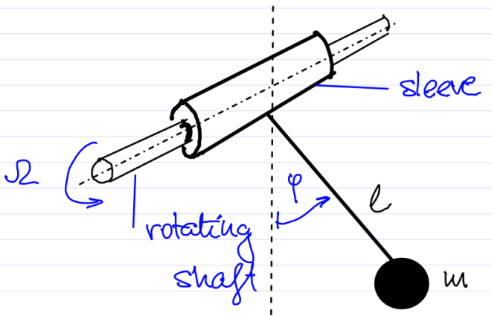
\includegraphics[width=0.4\textwidth]{figures/ch2/27friction_pend.png}
	\caption{The setup of the friction pendulum.}
	\label{fig:friction_pend}
\end{figure}
The torque driving the pendulum is given by 
\begin{align}
	T(\dot{\varphi}) = T_0  \textrm{sign}(\Omega - \dot{\varphi}).
\end{align}
From this we get the equation of motion
\begin{align}
	ml^2 \ddot{\varphi} + mgl \sin(\varphi) = T(\dot{\varphi}) = T_0  \textrm{sign} (\Omega - \dot{\varphi}).
\end{align}
By assuming $\Omega \gg 1$, i.e. very fast rotation of the shaft, we find that $T(\dot{\varphi}) = T_0$. Next we transform the coordinates in order to get an ODE
\begin{align}
	\begin{pmatrix}
		x_1 \\ x_2
	\end{pmatrix}
	=
	\begin{pmatrix}
		\varphi \\ \dot{\varphi}
	\end{pmatrix}
	;\quad
	\begin{pmatrix}
		\dot{x}_1 \\ \dot{x_2}
	\end{pmatrix}
=
\begin{pmatrix}
	x_2 \\ - \frac{g}{l} \sin(x_1) + \frac{T_0}{ml^2}
\end{pmatrix}
.
\end{align}
Thus the fixed point $x_0$ is at $(\overline{x}_1, \overline{x}_2)$ given by 
\begin{align}
	\sin(\overline{x}_1) = \frac{T_0}{mgl};\quad \overline{x}_2=0.
\end{align}
Since the system is forced, energy is not conserved and we cannot use it as a Lyapunov function. However, there may still exist a conserved quantity. Consider using
\begin{align}
	V(x) = \left[  \textrm{total energy at time } t \right] - \left[  \textrm{work put in between time } t  \textrm{ and } t_0 \right] = \left[ \textrm{initial energy} \right] =  \textrm{const.}  
\end{align}
This is a conserved quantity in all mechanics problems, but generally cannot be calculated without already knowing the trajectories. Here we can, as
\begin{align}
	V(x(t)) = \frac{1}{2} ml x_2^2 + mgl(1- \cos(x_1)) - T_0(\underbrace{x_1}_{\varphi(t)} - \underbrace{x_1(0)}_{\varphi(0)}).
\end{align}
We can drop the constant term $T_0 x_1(0)$. Now verify that $V$ is indeed constant
\begin{align}
	\dot{V}(x) = \frac{\partial V}{\partial x_1} \dot{x}_1 + \frac{\partial V}{\partial x_2} \dot{x}_2 = \left( mgl \sin(x_1) - T_0\right) x_2 + ml^2x_2 \left( - \frac{g}{l}\sin(x_1) + \frac{T_0}{ml^2} \right) = 0.
\end{align}
Hence $\dot{V}(x)$ is semidefinite, and may be used to conclude stability or instability. We must check the Lyapunov conditions for $V(x)$ 
\begin{subequations}
\begin{align}
	DV(x_0) &= 
\begin{pmatrix}
	mgl \sin(\overline{x}_1) - T_0 & ml^2 \overline{x}_2
\end{pmatrix}
=
\begin{pmatrix}
	0& 0
\end{pmatrix}
\\
D^2V(x_0) &= 
\begin{pmatrix}
	mgl \cos(\overline{x}_1) & 0 \\
	0 & ml^2
\end{pmatrix}.
\end{align}\end{subequations}
The Hessian is positive definite as long as $\overline{x}_1 \in \left(-\frac{\pi }{2}, \frac{\pi }{2}\right)$, and all fixed points in this region are stable by Theorem \ref{thm:direct}. The Hessian is indefinite if $\overline{x}_1 \not \in \left[-\frac{\pi }{2}, \frac{\pi }{2}\right]$, but in this case Theorem 4 is not applicable as $\dot{V}$ is not definite. More detailed discussion and further results on Lyapunov's direct method can be found in \cite{LiapunovDirect}.
 \end{ex}
 
